\documentclass[fontscale=0.35,landscape,paperwidth=841mm,paperheight=1189mm]{baposter}  % fontscale=0.285, dvipdfm

\usepackage{setspace}
\usepackage{multicol}
\usepackage{multirow}

\usepackage{tikz}
\usetikzlibrary{shapes,arrows} %for flowchart
% Define block styles
\newcommand{\flowchartscale}{0.6}
\tikzstyle{decision} = [diamond, draw, fill=iumint, 
    text width=5em, text badly centered, node distance=3cm, inner sep=0pt,
	 font=\diagsans, scale=\flowchartscale]
\tikzstyle{block} = [rectangle, draw, fill=iulimestone, 
    text width=5em, text centered, rounded corners, minimum height=4em,
	 font=\diagsans, scale=\flowchartscale]
\tikzstyle{line} = [draw, -latex', thick, font=\diagsans]
\tikzstyle{cloud} = [draw, ellipse,fill=iumidnight, text=grey, text width=8em,
	text centered, %node distance=3cm,
	minimum height=2em, font=\diagsans, scale=\flowchartscale]
%\usepackage{pgfbaselayers}
%\pgfdeclarelayer{background}
%\pgfdeclarelayer{foreground}
%\pgfsetlayers{background,main,foreground}

\tikzset{
  every overlay node/.style={
    draw=none,fill=none,rounded corners,anchor=north west,
  },
}
% Usage:
% \tikzoverlay at (-1cm,-5cm) {content};
% or
% \tikzoverlay[text width=5cm] at (-1cm,-5cm) {content};
\def\tikzoverlay{%
   \tikz[baseline,overlay]\node[every overlay node]
}%


%%% Color Definitions %%%%%%%%%%%%%%%%%%%%%%%%%%%%%%%%%%%%%%%%%%%%%%%%%%%%%%%%%

\selectcolormodel{cmyk}

\definecolor{bordercol}{RGB}{0,0,0}
%\definecolor{headercolone}{RGB}{6,130,22}
\definecolor{headercol}{cmyk}{1,0.64,0,0.6}
%\definecolor{headercolone}{cmyk}{1,0.64,0,0.6}
%\definecolor{headercoltwo}{cmyk}{0.44,0,0.15,0.17}
%\definecolor{headercolone}{cmyk}{0.3,0,0.15,0.17}
%\definecolor{headercoltwo}{cmyk}{0.3,0,0.15,0.17}
\definecolor{iumint}{cmyk}{0.40,0,0.23,0}
\definecolor{iumidnight}{cmyk}{0.71,0.30,0.13,0.41}
\definecolor{iulimestone}{cmyk}{0.11,0.13,0.14,0.26}
\definecolor{tuvagold}{cmyk}{0.0,0.2,1.0,0.0}
\definecolor{tuvablue}{cmyk}{0.57,0.23,0.0,0.1}
\definecolor{boxcolor}{RGB}{176,208,223}
%\definecolor{boxcolor}{cmyk}{0.3,0.08,0.08,0.1}
%\definecolor{boxcolor}{cmyk}{0.2,0.03,0.03,0.1}
%\definecolor{boxcolor}{cmyk}{0.57,0.23,0.0,0.1}
\definecolor{headerfontcol}{RGB}{255,255,255}
\newcommand{\hilitetwo}[1]{{\addfontfeature{Color=99333399}#1}}
\newcommand{\hiliteone}[1]{{\addfontfeature{Color=06821699}#1}}
\newcommand{\hilitegrey}[1]{{\addfontfeature{Color=77777799}#1}}
\newcommand{\hilitelightgrey}[1]{{\addfontfeature{Color=CCCCCC99}#1}}
\newcommand{\hiliteblue}[1]{{\addfontfeature{Color=44697DFF}#1}}
\newcommand{\hilitegold}[1]{{\addfontfeature{Color=tuvagold}#1}}

%%% Utility functions %%%%%%%%%%%%%%%%%%%%%%%%%%%%%%%%%%%%%%%%%%%%%%%%%%%%%%%%%%

%%% Save space in lists. Use this after the opening of the list %%%%%%%%%%%%%%%%
\newcommand{\compresslist}{
        \setlength{\itemsep}{1pt}
        \setlength{\parskip}{0pt}
        \setlength{\parsep}{0pt}
}

\usepackage{polyglossia}
\setdefaultlanguage[variant=australian]{english}

\usepackage{expex}

\usepackage{fontspec}
\defaultfontfeatures{PunctuationSpace=2,Scale=MatchLowercase,Mapping=tex-text}
\newfontfeature{IPA}{+mgrk}
%\setromanfont[IPA]{FreeSerif}
%\setromanfont[IPA,Scale=0.8]{CMU Serif}
%\setromanfont[IPA]{Liberation Serif}
%\setromanfont[IPA]{Linux Libertine O}
%\setromanfont[IPA]{Linux Biolinum O}
\setromanfont[IPA,Scale=1.01]{PT Sans}
%\setromanfont[IPA]{Nimbus Roman No9 L}
\setmonofont[IPA]{DejaVu Sans Mono}
\usepackage[small,bf]{caption}
%\newfontfamily\qipa[IPA,Scale=MatchLowercase]{FreeSerif}
\newfontfamily\qipa[IPA,Scale=MatchLowercase]{FreeSans}
\newfontfamily\qgmk[IPA,Scale=0.8]{CMU Serif}
\newfontfamily\litamono[IPA,Scale=0.5]{DejaVu Sans Mono}
\newfontfamily\ortamono[IPA,Scale=0.625]{DejaVu Sans Mono}
\newfontfamily\ortaqmono[IPA,Scale=0.75]{DejaVu Sans Mono}
\newfontfamily\diagsans[IPA,Scale=1]{DejaVu Sans}

\newcommand{\tilda}{{\qipa ∼}}

\newcommand{\tags}[1]{\hiliteone{#1}}
\newcommand{\tag}[1]{{\ortaqmono \hilitegrey{<}\hiliteblue{#1}\hilitegrey{>}}}
\newcommand{\archiphon}[1]{\hilitegrey{\{}\hiliteone{#1}\hilitegrey{\}}}

%\newfontfamily\htwo[IPA,Scale=1.2]{FreeSans}}
%\newfontfamily\htwofont[IPA,Scale=1]{CMU Sans Serif}
%\newfontfamily\htwofont[IPA,Scale=1,Color=333344FF]{CMU Sans Serif}
\newfontfamily\htwofont[IPA,Scale=1,Color=111111FF]{CMU Sans Serif}
%\newfontfamily\titlefont[IPA,Scale=0.52]{CMU Serif}
%\newfontfamily\titlefont[IPA,Scale=0.7]{CMU Serif}
%\newfontfamily\titlefont[IPA,Scale=0.7]{CMU Sans Serif Demi Condensed}
\newfontfamily\titlefont[
	%SmallCapsFont={Andika},
	%SmallCapsFont={Alegreya Sans SC},
	SmallCapsFont={Andada SC},
	%SmallCapsFont={Carrois Gothic SC},
	SmallCapsFeatures={Letters=SmallCaps},
	Scale=0.8,
]{Andada SC}
%\newfontfamily\titlefont[IPA,Scale=0.7]{Nimbus Sans L}
%\newfontfamily\titlefont[IPA,Scale=0.55]{DejaVu Serif}

%\newcommand{\htwo}[1]{::: {\htwofont #1} :::}%\hrule} %\hline\\}
%\newcommand{\htwo}[1]{{\htwofont \textbf{:::#1:::}}}%\hrule} %\hline\\}
%\newcommand{\htwo}[1]{{\htwofont \textbf{\hilitegold{\dotfill{}}#1\hilitegold{\dotfill{}}}}}
\newcommand{\htwo}[1]{{\htwofont \textbf{\dotfill{}#1\dotfill{}}}}
\newcommand{\dividerspace}{\vspace{0.5em}}


\usepackage{graphicx}  % [dvipdfm]

%\definecolor{MyGray}{rgb}{0.96,0.97,0.98}
%\newenvironment{codebox}{%
%   \begin{lrbox}{\@tempboxa}\begin{minipage}{\columnwidth}}{\end{minipage}\end{lrbox}%
%   \colorbox{MyGray}{\usebox{\@tempboxa}}
%}
%\newcommand{\codeex}[1]{\begin{codebox}#1\end{codebox}}

%\definecolor{grey}{rgb}{0.96,0.97,0.98}
\definecolor{grey}{rgb}{0.91,0.91,0.91}
\newcommand{\codeex}[1]{
   \fbox{\colorbox{grey}{
         \begin{minipage}[t]{0.91\textwidth}{\litamono
				\begin{spacing}{0.4}
	            #1
				\vspace{-1em}\end{spacing}
         }\end{minipage}
      }
   }
}
\newcommand{\outputex}[1]{
   \fbox{\colorbox{iumidnight}{
         \begin{minipage}[t]{0.91\textwidth}{\ortamono
				\begin{spacing}{0.2}\vspace{-0.8em}
	            \hilitelightgrey{#1}
				\vspace{-2.5em}\end{spacing}
         }\end{minipage}
      }
   }
}



\newcommand{\blank}[1]{\underline{\hspace{#1}}}

%\usepackage{natbib}
\usepackage[backend=biber,citestyle=apa,maxcitenames=2,style=authoryear,maxbibnames=99,uniquelist=false,uniquename=false]{biblatex}
\bibliography{poster}
\renewcommand*{\nameyeardelim}{\addcomma\space}
\renewcommand*{\bibfont}{\fontsize{5.75pt}{5.75pt}\selectfont}
\renewcommand*{\intitlepunct}{\space}


\usepackage[colorlinks=true,citecolor=black,linkcolor=black,urlcolor=black]{hyperref}

\usepackage{subfigure}
\usepackage{booktabs}

%%\bibpunct{(}{)}{;}{A}{,}{,}
%\bibdata{paper}

%\newcommand{\citemultileft}[1]{(\citeauthor{#1}, \citeyear{#1}}
%\newcommand{\citemultimid}[1]{\citeauthor{#1}, \citeyear{#1}}
%\newcommand{\citemultiright}[1]{\citeauthor{#1}, \citeyear{#1})}
%\newcommand{\citetwoyears}[2]{\citeauthor{#1} (\citeyear{#1} and \citeyear{#2})}

% for glosses
\newcommand{\eng}[1]{`{\em #1}'}
%dammit, sc doesn't seem to be working
\newcommand{\gmk}[1]{{\qgmk \textsc{#1}}}


\usepackage{enumitem}
\setlist{nolistsep,leftmargin=*}
\newenvironment{itemise}[1]{
        \begin{itemize}\setlength{\leftmargin}{-4em}\setlength{\itemsep}{-0.2em}
        \vspace{-0.5em}
        #1
}{
        \end{itemize}
        \vspace{-2pt}
}

%\newcommand{\h2}[1]{{\big



\begin{document}
	% To get it to be the same size consistently on all machines..
	\special{papersize=841mm,1189mm}
	\setlength{\pdfpageheight}{\paperheight}
	\setlength{\pdfpagewidth}{\paperwidth}

	%%% Setting Background Image %%%
	%\background{}

	\begin{poster}{
		grid=false,
		%eyecatcher=false,
		borderColor=bordercol,
		headerColorOne=iumidnight,
		headerColorTwo=iumidnight,
		%headerColorOne=blue,
		headerFontColor=tuvagold,
		% Only simple background color used, no shading, so boxColorTwo isn't necessary
		boxColorOne=boxcolor,
		headershape=roundedright,
		headerborder=open,
		headerheight=0.07\textheight,
		%headershape=roundedright,
		%headershade=plain,
		%headerfont=\Large\textsf, %Sans Serif
		%headerfont=\Large\sf\bf,
		textborder=rectangle,
		%background=plain,
		%background=user,
		background=none,
		headerborder=open,
		boxshade=plain,
		textborder=roundedleft,
		columns=3,
	}{ %Eye Catcher, empty if option eyecatcher=false - unused
		\setlength\fboxsep{0.5em}
		\setlength\fboxrule{0pt}
		%\includegraphics[angle=90,height=6.2em]{apertium5b}%\hspace{-2em}
		\includegraphics[height=5.8em]{uitlogo}\hspace{1em}
		\fbox{\includegraphics[height=5.4em]{iu_tab-crop}}
		%\hspace{2.5cm}\begin{minipage}[t]{7em}
		%	\vspace{-2cm}
		%	\noindent\\
		%	\vspace{-0.5ex}\hspace{0.105cm}
		%\end{minipage}

	}{ %Title (centered top)
		{%\vspace{0pt}\hspace{1cm} \
			{\titlefont \scshape{A finite-state morphological analyser for Tuvan}
			}
		}
	}{ %Authors (centered top, below title)
		%\vspace{-0.6em}
		\begin{center}
			\begin{minipage}[t]{8.5em} %{7em}
				\begin{spacing}{0.4}
				{Francis M.\ Tyers}\\
				{\footnotesize UiT Norgga Árktalaš Universitehta \\\texttt{francis.tyers@uit.no}}
				\end{spacing}
			\end{minipage}
			\begin{minipage}[t]{12em}
				\begin{spacing}{0.4}
					{Jonathan North Washington}\\
					{\footnotesize Indiana University\\\texttt{jonwashi@indiana.edu}}
				\end{spacing}
			\end{minipage}
			\begin{minipage}[t]{9em} %{7.7em}
				\begin{spacing}{0.4}
					{Aziyana Bayyr-ool}\\
					{\footnotesize Сибирское отделение Российской академии наук,~~\texttt{azikoa@mail.ru}}
				\end{spacing}
			\end{minipage}
			\begin{minipage}[t]{8em} %{6em}
				\begin{spacing}{0.4}
					{Aelita Salchak\vphantom{y}}\\
					{\footnotesize Тываның Күрүне Университеди\\\texttt{aelita\_74@mail.ru}}
				\end{spacing}
			\end{minipage}
		\end{center}
	}{ %More eye catchers, on the right side
		\setlength\fboxsep{0.5em}
		\setlength\fboxrule{0pt}
		\fbox{
\includegraphics[height=5.5em]{img/Tuvsu}}
		
\includegraphics[height=5.4em]{img/soranif}
		%\hspace{2.5cm}
	}

	\headerbox{Tuvan}{name=tyvan,column=0,row=0}{
		\includegraphics[width=\textwidth]{img/tuvanmap}
		\tikzoverlay[text width=1in] at (2.5in, -0in) {
			\includegraphics[width=1in]{img/Flag_of_Tuva}
		};
		\vspace{-1.2em}
		\begin{itemize}
			\item Sayan Turkic language
			\item Spoken in the Tuva Republic
			\item Approximately 300,000 speakers
			\item Agglutinative morphology
			\item Very little work on computational tools
		\end{itemize}
	}
	
	\headerbox{Morphological Transducers}{name=morphtrans,below=tyvan}{
		\htwo{Morphological transducers}
		\begin{itemize}
			\item Efficient (in speed \& size) models of a language's morphology
			\item Take a surface form, and produce valid lexical form(s)
			\item Take a lexical form, and produce valid surface form(s)\vspace{-0.1ex}\\
		%\end{itemize}
		%\scalebox{0.98}{
			алдым\hfill{}{\qipa \hilitetwo{↔}}\hfill{}\texttt{ал\tag{v}\tag{tv}\tag{ifi}\tag{p1}\tag{sg}},~~\texttt{алд\tag{n}\tag{px1sg}\tag{nom}}\\
			өөнде\hfill{}{\qipa \hilitetwo{↔}}\hfill{}\texttt{өг\tag{n}\tag{px3sp}\tag{loc}}
		%}
		\end{itemize}
		\dividerspace{}

		\htwo{Framework:\ HFST}
		\begin{itemize}
			\item Reimplements Xerox FST formalisms ({\tt lexc} \& {\tt twol})
			\item Also provides a wrapper around popular free/open-source FST toolkits: SFST, OpenFST, and Foma
		\end{itemize}
		\dividerspace{}

		\htwo{Approach}
		\begin{itemize}
			\item two-level method \parencite{koskenniemi83}
			\item \textbf{morphotactics} implemented in \texttt{lexc}
			\item \textbf{morphophonology} implemented in \texttt{twol} (SPE-style rules)
			\item compiled separately; compose-intersected to single transducer\vspace{-0.1ex}\\
			алдым\hfill{}{\qipa \hilitetwo{↔}}\hfill{}\texttt{ал\hilitegrey{>}\archiphon{D}\archiphon{I}\hilitegrey{>}м}\hfill{}{\qipa \hilitetwo{↔}}\hfill{}\texttt{ал\tag{v}\tag{tv}\tag{ifi}\tag{p1}\tag{sg}}\vspace{-0.1ex}\\
			алдым\hfill{}{\qipa \hilitetwo{↔}}\hfill{}\texttt{алд\hilitegrey{>}\archiphon{I}м}\hfill{}{\qipa \hilitetwo{↔}}\hfill{}\texttt{алд\tag{n}\tag{px1sg}\tag{nom}}\\
			өөнде\hfill{}{\qipa \hilitetwo{↔}}\hfill{}\texttt{өг\hilitegrey{>}\archiphon{z}\archiphon{I}\archiphon{n}\hilitegrey{>}\archiphon{D}\archiphon{A}}\hfill{}{\qipa \hilitetwo{↔}}\hfill{}\texttt{өг\tag{n}\tag{px3sp}\tag{loc}}
		\end{itemize}

	}


	\headerbox{Finding out new linguistics things}{name=harglebargle,column=0,below=morphtrans}{
		\begin{center}
		\begin{tabular}{lllll}
		\toprule
			stem & V & C & dative & genitive \\
		\midrule
			медаль & а & ль & медальг\hiliteone{а} & медальд\hiliteone{ы}ң \\
			ансамбль & а & бль & ансамбльг\hilitetwo{е} & ансамбльд\hilitetwo{и}ң \\\midrule
			руль & у & ль & рульг\hiliteone{а} & рульд\hiliteone{у}ң \\
			рубль & у & бль & рубльг\hilitetwo{е} & рубльд\hilitetwo{и}ң \\
		\bottomrule
		\end{tabular}
		\end{center}\vspace{-0.5em}
\codeex{\hilitegrey{"\{I\} harmony"\\
	\%\{I\%\}:Vy <=> :Vx [ :Cns* :RealCns ]/[ :0 | \%- ]* \_ ;}\\
	\-~~~~~~~~~except\\
	\-~~~~~~~~~~~~~[ :BackVow :Cns* :Cns :л ь: :Cns* :RealCns ]/:0* \_ ;\\
	\-~~~~~~~~~~~~~[ :BackVow :Cns* :Cns :л ь:0 ]/:[ :0 - ь: ]* \_ ;\\
	\-~~~~~~~~~\hilitegrey{where Vx in ( ү и е э ө а о ы у я ё ю )\\
	\-~~~~~~~~~~~~~~ Vy in ( ү и и и ү ы у ы у ы у у )\\
	\-~~~~~~~~~matched ;}\\
	\\
	"\{I\} always front when intervening Cль"\\
	\%\{I\%\}:и <=> [ :BackVow :Cns* :Cns :л ь: :Cns* :RealCns ]/:0* \_ ;\\
	\-~~~~~~~~~~~~[ :BackVow :Cns* :Cns :л ь:0 ]/:[ :0 - ь: ]* \_ ;}
	}


		\headerbox{Development cycle}{name=development,below=harglebargle,span=1}{
		\centering
		\begin{tikzpicture}[xscale=1.45,yscale=2.2]%, auto]

			\node[cloud] (assumptions) at (1,2.75) {assumed generalisations};
			\node[block] (compile) at (1,2) {compile analyser};
			\node[block] (analyse) at (1,1.4) {analyse corpus};
			\node[block] (check) at (1,0.7) {examine freq.\ list};
			\node[decision] (missingstem) at (1,0) {missing stem?};
			\node[block] (addstem) at (0,2) {add stem};
			\node[decision] (phonormorph) at (2.25,0) {type of problem?};
			\node[block] (updatephon) at (3.5,0) {update phonol.};
			\node[block] (updatemorph) at (3.5,1) {update morphol.};
			\node[decision] (phonbetter) at(5,0) {better?};
			\node[decision] (morphbetter) at (5,1) {better?};
			\node[cloud] (newgeneralisation) at (3,2) {new\\grammatical\\generalisation};

			\path[line] (assumptions) -- node [right=0.75ex, align=left, scale=\flowchartscale] {initial\\development} (compile);
			\path[line] (compile) -- (analyse);
			\path[line] (analyse) -- node [right=0.75ex, scale=\flowchartscale, align=left] {unanalysed\\forms} (check);
			\path[line] (check) -- (missingstem);
			\path[line] (missingstem) -| node [below=1ex, near start, scale=\flowchartscale] {yes} (addstem);
			\path[line] (addstem) -- (compile);
			\path[line] (missingstem) -- node [below=1ex, midway, scale=\flowchartscale] {no} (phonormorph);
			\path[line] (phonormorph) -- node [below=1ex, near start, scale=\flowchartscale] {phon} (updatephon);
			\path[line] (phonormorph) |- node [below=1ex, near end, scale=\flowchartscale] {morph} (updatemorph);
			\path[line] (updatephon) -- node [above=0.5ex, scale=\flowchartscale, align=center] {diff \\ freq list} (phonbetter) ;
			\path[line] (updatemorph) -- node [above=0.5ex, scale=\flowchartscale, align=center] {diff \\ freq list} (morphbetter) ;
			\path[line] (phonbetter.east) -- node [below=1ex, near start, scale=\flowchartscale] {yes} (5.6,0) |- (newgeneralisation.east) ;
			\path[line] (morphbetter.east) -- node [below=1ex, near start, scale=\flowchartscale] {yes} (5.6,1) |- (newgeneralisation.east) ;
			\path[line] (phonbetter.north) |- node [right=1ex, near start, scale=\flowchartscale] {no} (5,0.5) -| (updatephon.north) ;
			\path[line] (morphbetter.north) |- node [right=1ex, near start, scale=\flowchartscale] {no} (5,1.5) -| (updatemorph.north) ;
			\path[line] (newgeneralisation) -- (compile);

		\end{tikzpicture}
%			\begin{tikzpicture}[xscale=1.92,yscale=2.65]%, auto]	
%
%				\node[cloud] (assumptions) at (1,2.75) {assumed generalisations};
%				\node[block] (compile) at (1,2) {compile analyser};
%				\node[block] (analyse) at (1,1.5) {analyse corpus};
%				\node[block] (check) at (1,1) {examine freq.\ list};
%				\node[decision] (missingstem) at (1,0) {missing stem?};
%				\node[block] (addstem) at (0.22,2) {add stem};
%				\node[decision] (phonormorph) at (2,0) {type of problem?};
%				\node[block] (updatephon) at (3,0) {update phonol.};
%				\node[block] (updatemorph) at (3,1) {update morphol.};
%				\node[decision] (phonbetter) at( 4,0) {better?};
%				\node[decision] (morphbetter) at (4,1) {better?};
%				\node[cloud] (newgeneralisation) at (2.5,2) {new\\grammatical\\generalisation};
%
%				\path[line] (assumptions) -- node [right=0.75ex, align=left, scale=\flowchartscale] {preliminary\\development} (compile);
%				\path[line] (compile) -- (analyse);
%				\path[line] (analyse) -- (check);
%				\path[line] (check) -- node [right=0.75ex, scale=\flowchartscale, align=left] {unanalysed\\forms} (missingstem);
%				\path[line] (missingstem) -| node [below=1ex, near start, scale=\flowchartscale] {yes} (addstem);
%				\path[line] (addstem) -- (compile);
%				\path[line] (missingstem) -- node [below=1ex, midway, scale=\flowchartscale] {no} (phonormorph);
%				\path[line] (phonormorph) -- node [below=1ex, near start, scale=\flowchartscale] {phon} (updatephon);
%				\path[line] (phonormorph) |- node [below=1ex, near end, scale=\flowchartscale] {morph} (updatemorph);
%				\path[line] (updatephon) -- node [above=0.5ex, scale=\flowchartscale, align=center] {diff \\ freq \\ list} (phonbetter) ;
%				\path[line] (updatemorph) -- node [above=0.5ex, scale=\flowchartscale, align=center] {diff \\ freq \\ list} (morphbetter) ;
%				\path[line] (phonbetter.east) -- node [below=1ex, near start, scale=\flowchartscale] {yes} (4.6,0) |- (newgeneralisation.east) ;
%				\path[line] (morphbetter.east) -- node [below=1ex, near start, scale=\flowchartscale] {yes} (4.6,1) |- (newgeneralisation.east) ;
%				\path[line] (phonbetter.north) |- node [right=1ex, near start, scale=\flowchartscale] {no} (4,0.5) -| (updatephon.north) ;
%				\path[line] (morphbetter.north) |- node [right=1ex, near start, scale=\flowchartscale] {no} (4,1.5) -| (updatemorph.north) ;
%				\path[line] (newgeneralisation) -- (compile);
%			\end{tikzpicture}%}

		}


	\headerbox{Example}{name=example,span=2,column=1,row=0}{
	{\centering
	{\fontsize{12pt}{12pt}\selectfont \em{« Бис кожууннуң соңгукчулары-биле ажылды чорутпастай бээривиске, көргүзүглер баксыраан. »}}\vspace{0.5em}\\
	{\fontsize{12pt}{12pt}\selectfont ``Figures worsened when we stopped conducting business with the district's constituents.''}\\
	%Когда мы перестали проводить работу с избирателями кожууна, показатели ухудшились
	}
	%\vspace{-1em}
	
		%\texttt{алд\hilitegrey{>}\archiphon{I}м}\hfill{}\hilitetwo{↔}\hfill{}\texttt{алд\tag{n}\tag{px1sg}\tag{nom}}
	\begin{multicols}{2}
	{\fontsize{14pt}{14pt}\selectfont
		\texttt{\textasciicircum Бис/бис\tag{prn}\tag{pers}\tag{p1}\tag{pl}\tag{nom}\$}\\
		\texttt{\textasciicircum кожууннуң/кожуун\tag{n}\tag{gen}\$}\\
		\texttt{\textasciicircum соңгукчулары/соңгукчу\tag{n}\tag{pl}\tag{px3sp}\tag{nom}\$}\\
		\texttt{\textasciicircum -биле/биле\tag{post}\$}\\
		\texttt{\textasciicircum ажылды/ажыл\tag{n}\tag{acc}\$}\\
		\texttt{\textasciicircum чорутпастай/чорут\tag{v}\tag{tv}\tag{cess}\tag{prc\_impf}\$}\\
		\texttt{\textasciicircum бээривиске/бер\tag{vaux}\tag{ger\_aor}\tag{px1pl}\tag{dat}\$}\\
		\texttt{\textasciicircum ,/,\tag{cm}\$}\\
		\texttt{\textasciicircum көргүзүглер/көргүзүг\tag{n}\tag{pl}\tag{nom}\$}\\
		\texttt{\textasciicircum баксыраан/баксыра\tag{v}\tag{iv}\tag{past}\tag{p3}\tag{pl}\$}\\
		\texttt{\textasciicircum ./.\tag{sent}\$}}\\
		\tikzoverlay[text width=10em] at (3.3in, 0in) {
			Lexicon contents {\qipa ↗}
		};
		\columnbreak

		\hspace*{1in}\begin{tabular}{llr}
			\toprule
			Part of speech	&	Tag	& Stems \\
			\midrule
			Noun & \tag{n} & 4,226 \\
			Proper noun & \tag{np} & 4,217 \\
			Adjective & \tag{adj} & 1,603 \\
			Verb & \tag{v} & 1,064 \\
			Adverb & \tag{adv} & 136 \\
			Numeral & \tag{num} & 85 \\
			Conjunction & \tag{cnj*} & 70 \\
			Postposition & \tag{post} & 28 \\
			Pronoun & \tag{prn} & 35 \\
			Determiner & \tag{det} & 26 \\
			\midrule
			Total &  & 11,490 \\
			\bottomrule
		\end{tabular}\\

	\end{multicols}

	}

	%\headerbox{Lexicon}{name=lexicon,column=1,below=example}{
	%	%\resizebox{0.9\textwidth}{!}{
	%	%}
	%}
		\headerbox{Morphotactics}{name=morphotactics,column=2,below=example}{
			\begin{itemize}
				\item Introduction of quasi-derivational verbal morphotactics
				\item Combinatorics not previously documented
			\end{itemize}
			\centering
			\includegraphics[width=0.9\textwidth]{img/dibuix}

		}
	\headerbox{Evaluation}{name=results,column=2,below=morphotactics}{ %lexicon}{
		%\begin{multicols}{2}	
		\htwo{5-part corpus for naïve coverage}
		\vspace{-0.2em}
		%\begin{itemize}
		%	\item Naïve coverage calculated on 5-part corpus
		%\end{itemize}
		\begin{center}
		\resizebox{0.9\textwidth}{!}{
		\begin{tabular}{lrr}
			\toprule
			 \textbf{Domain} & \textbf{Tokens} & \textbf{Coverage} (\%) \\
			\midrule
			 News       & 1,539,459 &  95.73  \\
			 Religion   & 746,124 &  93.84 \\
			 Literature & 297,830 &  91.96  \\
			 Encyclopaedic  & 276,547 & 90.86 \\
			 Folklore & 27,902 & 91.57  \\\cline{2-3}
			 Average    & -- & 92.79 \\
			\bottomrule
		\end{tabular}}
		\end{center}

		\htwo{Precision and recall}
		\vspace{-0.2em}
		%\begin{itemize}
		%	\item Good results reflect high accuracy
		%\end{itemize}
		\begin{center}
		\resizebox{0.9\textwidth}{!}{
		\begin{tabular}{llrr}
			\toprule
				& \textbf{count} & \textbf{precision} & \textbf{recall} \\
			\midrule
			known tokens & 1024 & 0.99 & 0.97 \\
			all tokens & 1425 & 0.99 & 0.69 \\
			\bottomrule
		\end{tabular}}
		\end{center}
		%{\qipa ↑} quantitative eval\\
		%\newline
		%\vspace{0.01pt}\hfill{}qualitative eval {\qipa ↗}\\
		%\columnbreak
		
		\htwo{Qualitative evaluation}
		\vspace{-0.2em}
		%\begin{itemize}
		%	\item Qualitative evaluation
		%\end{itemize}

		\begin{center}
		\resizebox{0.9\textwidth}{!}{
		\begin{tabular}{lrr}
			\toprule
			\textbf{error type} & \textbf{count} & \textbf{percentage} \\
			\midrule
			Missing stem &  364 & 78.8 \\
			Other & 65 & 14.1  \\
			Bad morphotactics & 19 & 4.1  \\
			Bad phonology & 8 & 1.7  \\
			Incorrect categorisation & 6 & 1.3  \\
			\midrule
			Total: & 462 & 100 \\
			\bottomrule
		\end{tabular}}
		\end{center}

	%	\begin{tabular}{lr}
	%		\toprule
	%		error type & count \\
	%		\midrule
	%		Missing stem & 364 \\
	%		Other & 65 \\
	%		Bad morphotactics & 19 \\
	%		Bad phonology & 8 \\
	%		Incorrect categorisation & 6 \\
	%		\bottomrule
	%	\end{tabular}
		%\end{multicols}
		%\vspace{0.05em}

	}


		\headerbox{Ongoing and future work}{name=nedostatki,column=1,below=example}{
		\htwo{our other Turkic-language transducers}
		\begin{itemize}
			%\item Turkish (\hiliteone{Çöltekin, 2010 \& 2014}; \hilitetwo{Oflazer, 1994})
			%\item Crimean Tatar (\hilitetwo{Altıntaş, 2001})
			%\item Turkmen (\hilitetwo{Tantuğ et al., 2006})
			%\item Kazakh (\hilitetwo{Бекманова \& Махимов, 2013})
			%\vspace{1pt}\hfill{} \hiliteone{GPL (=free and open)}!
			%\item our Kyrgyz, Kazakh, Tatar, Kumyk:\ all \hiliteone{GPL (=free and open)}!
			\item \textbf{Kyrgyz} \parencite{jnwmifmt2012lrecpaper}%  (Washington et al., 2012)
			\item \textbf{Tatar} \& \textbf{Bashkort} \parencite{fmtjnwisrb2012lrecpaper} %(Tyers et al., 2012)
			\item \textbf{Kazakh} \parencite{isjnwfmt2013mtsummitpaper} %(Salimzyanov et al., 2013)
			\item \textbf{Kumyk} \parencite{jnwisfmt2014lrecpaper} %(Washington et al., 2014)
			\item ongoing work on Sakha, Khakas, and more!
		\end{itemize}
		\dividerspace{}

		\htwo{Morphological disambiguation}
		\begin{itemize}
			\item \textbf{Kazakh} \parencite{zajnwftanasakbada2016ciclingproceedings}
		\end{itemize}
		\dividerspace{}

		\htwo{Treebanks}
		\vspace{-1em}
		\newline
			\tikzoverlay[text width=0.9\textwidth] at (0.55in, -1in) {
				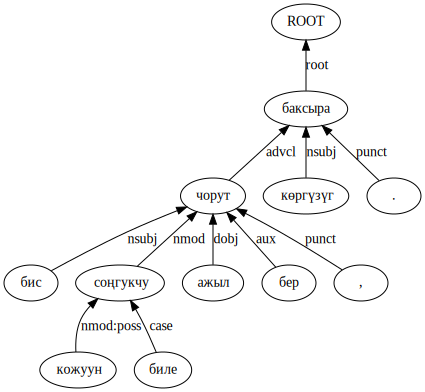
\includegraphics[width=0.95\textwidth]{img/dep-graph}
			};
		\begin{itemize}
			\item \textbf{Kazakh} \parencite{fmtjnw2015kazdep}
			\item work on \textbf{Tuvan} ongoing
		\end{itemize}
		\includegraphics[width=0.63\textwidth]{img/korp-2}
		%\begin{itemize}
		%\end{itemize}
		\vspace{1.55in}
		\dividerspace{}


		%\begin{itemize}

				%\item Current annotation of a dependency treebank for Kazakh:\\
				%a similar process that helps identify errors in morphological analyses and automatic disambiguation (constraint grammar)
				%%\item Leading to
				%\begin{itemize}
				%	\item Improved rule-based morphological disambiguation% (constraint grammar)
				%	\item Improved morphological analyser %for Kazakh
				%	\item A syntactic dependency treebank %for Kazakh
				%\end{itemize}
				%%\item Work on rule-based morphological disambiguation with constraint grammar
			%\end{itemize}
			\htwo{Future work}
				\begin{itemize}
					%\item Annotate more gold standard text in more Turkic languages
					%\item Research cross-linguistic techniques for analysing Turkic
					\item Dependency parsing (native and crosslingual)
					\item Increase number of stems
					\item Make more available to linguists
					\item Integrate into end-user applications (spellchecking, MT)
				\end{itemize}
				%\item Disambiguation, more stems, clean up transducers
				%\item Machine translation between these languages
				%\item Bring other Kypchak transducers to comparable performance:\\
				%Qaraqalpaq, Bashqort, Nogay, Crimean Tatar
				%\item Other Turkic lgs:\ Uzbek, Uyghur, Chuvash, Yakut, Tuvan, etc.
				\includegraphics[width=\textwidth]{img/tyv-spelling}
		}

	\headerbox{References}{name=references,below=results,column=2}{
		\vspace{-0.42em}
		\begin{spacing}{0.3}
			\printbibliography[heading=none]
		\end{spacing}
		\vspace{-0.05em}
	}


		\headerbox{Further information}{name=getting,column=0,below=development,span=3}{
			\tikzoverlay[text height=1in] at (0in, 0.04in) {
				\includegraphics[angle=90,height=1in]{apertium5b}
			};
			%\tikzoverlay[text width=0.8in] at (6.2in, 0.04in) {
			\tikzoverlay[text height=1in] at (10in, 0.04in) {
				\includegraphics[height=1in]{qrcode}
			};
			\tikzoverlay[text height=0.5in] at (6.75in, 0in) {
				\parbox{3in}{
				\centering
				{\huge \textbf{Четтирдивис!}}\\
				\texttt{четтир\tag{v}\tag{tv}\tag{ifi}\tag{p1}\tag{pl}}\vspace{1em}\\
				{\Large \url{http://turkic.apertium.org/}}
				}
			};
			\tikzoverlay[text width=6in] at (1in, 0.04in) {
			\begin{itemize}
				\item Part of \textbf{Apertium Turkic} project:\ \url{http://wiki.apertium.org/wiki/Apertium\_Turkic}
				\item Transducers available \textbf{live} on our website: \url{http://turkic.apertium.org/} %\href{http://turkic.apertium.org/}{\texttt{turkic.apertium.org}}
				\item \textbf{Source code} under \hiliteone{GPL} from Apertium's SVN repo
				%\item Transducers available \textbf{live} at \href{http://turkic.apertium.org/}{\texttt{turkic.apertium.org}}
				%\item \textbf{Source code} of transducers available under \hiliteone{GPL} (free!) from Apertium's SVN repo
				%info at {\small \url{http://wiki.apertium.org/wiki/apertium-kir}}
				\item Multilingual Turkic RBMT \textbf{mailing list} (>25 subscribers):\ \texttt{apertium-turkic@lists.sourceforge.net}%\\
				%\vspace{-0.5ex}Feel free to post in any language!\\\vspace{-2.5ex}
				\item And feel free to contact the authors any time!
			\end{itemize}
			\vspace{0.3em}
			};
			\vspace{1in}
		}


	\end{poster}
\end{document}
